\documentclass{standalone}

\begin{document}

\subsection[Results]{Results}\label{obj_detection:results}

The original implementation of the YOLO model was provided by Redmon et al. and it is public available in his official \href{https://pjreddie.com/darknet/yolo}{web page} of \emph{Darknet project}.
The code is written in Ansi C and it is designed and, only thank to the many branches developed by the Github community, it can be compiled on all the OS.
The Ansi C language is a very low level programming language and it is hard to obtain better performances rewriting the code.
This guaranteed its supremacy in terms of speed in the research community.
The code is particularly optimized for GPU applications: the \emph{darknet} library provides an efficient CUDA support and thus can be optimally used only in NVIDIA GPUs.

The proposed \textsf{Byron} library was developed following the backbone and the innovative ideas into the \emph{Darknet} project.
The main difference between them is the programming language chosen: \textsf{Byron} is written in pure C++, a \quotes{higher} level programming language.
Generally we can not obtain better computational performances using C++ in relation to an Ansi C implementation.
However, the C++ language is more popular than Ansi C and more easy to write and modify.
The second main difference of \textsf{Byron} is related to the target computational environment: it is designed and optimized to reach the better performances on a single or multiple CPUs architecture.
In this way we can enlarge also the use of our code.
Many research groups, in fact, have very powerful server grade machines without the GPU support and it is hard for them to get close to the deep learning applications.
An emblematic case is given by the bioinformatic research in which a wide amount of money are spent to buy efficient server grade machines to process large set of DNA datasets which are commonly processed using only CPUs support.

In the previous sections we have discussed about different kind of optimization related to the various (possible) components of a Neural Network model.
All these optimizations were implemented in the \textsf{Byron} library to reach the best performances.
Moreover, studying the Redmon et al. implementation, many issues were found in the \emph{Darknet} project, especially in relation to the multi-threading support and the related thread concurrency.
The \textsf{Byron} library widely uses the OpenMP library paying attention to the thread concurrency and to the minimization of the time for threads spawning.
In \textsf{Byron} a single parallel section is open at the beginning of the processing and it is closed at the end, with a carefully management of the threads along all the network structure.

In view of these considerations a first test was performed to compare the \textsf{Byron} efficiency against the \emph{Darknet} one in terms of time performances.
To compare the results we implemented the same YOLO model into our custom \textsf{Byron} library and we compared its time efficiency against the original implementation.
The test were performed turning off the multi-threading support since the \emph{Darknet} implementation use it only in the GEMM evaluation.
We performed 5 independent simulations using the same input image size to test the time stability of both the implementations.
Each simulation performs 100 runs of both the algorithms.
The results are shown in Fig.~\ref{fig:yolo_time} where we normalized our times in relation to the \emph{Darknet} ones since it is our reference.

\begin{figure}[htbp]
\centering
\def\svgwidth{0.85\textwidth}
\input{./img/byron_timing.pdf_tex}
\caption{Comparison of time performances between the \textsf{Byron} and \emph{Darknet} implementations of the YOLO model.
The simulations were performed keeping fixed the input image sizes and without the multi-threading support.
Each simulation includes 100 runs of both the algorithms.
The \textsf{Byron} version is approximately 3.8x faster than \emph{Darknet} in all the simulations.
}
\label{fig:yolo_time}
\end{figure}

Both the implementations are quite stable across the simulations and our measures shows a very tight variability.
The differences in time performances are evident and we can summarized them with a 3.8x speedup obtained by the \textsf{Byron} implementation against the \emph{Darknet} one.
The multiple optimizations discussed and used by the \textsf{Byron} library are proofed by numerical results and highlights the efficiency of our implementation against the state-of-art.
We would stress also that using our version of the model into a server grade machine (128~GB RAM memory and 2 CPU E5-2620, with 8 cores each) the YOLO model can process $416\times416$ images in real-time (less than a second) while the \emph{Darknet} one could reach the same performances only with a GPU support.

Once the efficiency was proved we \quotes{update} the YOLO model to overcome its issues.
In particular, we have discussed in the previous section (ref. \ref{obj_detection:yolo}) that a big issue related to the YOLO model concerns the detection of small objects.
Despite the model is incredibly efficient in object detection also with low quality images, there is a sort of limit in the number of pixels needed for object identification.
This kind of problems are particularly critical in people detection and moreover in crowd counting applications.
YOLO is able to identify the major part of the persons into an image but it decreases its efficiency when they partly overlap or are far from the camera (and thus at low resolution).

We had the opportunity to empirically verify its limit working on a people tracking project for real time applications.
The project was developed in collaboration with the Complex Systems (\emph{PhySyCom}) group of the University of Bologna, with the support of Canon Inc., Telecom Italia and Fabbrica Digitale, and it aims to detect and track people using video camera devices.
The experiments were executed around the streets of Venice with the support of the Venice City Council.
Using our custom implementation of the YOLO model we were able to detect a large part of persons but we loose efficiency when the people flow increased or in open space area (a crucial point was Piazza San Marco).

In the previous section we largely discuss about the efficiency of Super Resolution techniques to improve the image quality so it stands to reason that the application of them will be helpful to overcome the told above issues.
To this purpose we apply the previously described EDSR model to the image which are not perfectly detected by the YOLO model.
For privacy reasons we cannot show the results obtained on the Venice data and thus we show a simple example to proof our model.
The example is shown in Fig.~\ref{fig:yolo_sr}.

\begin{figure}[htbp]
\centering
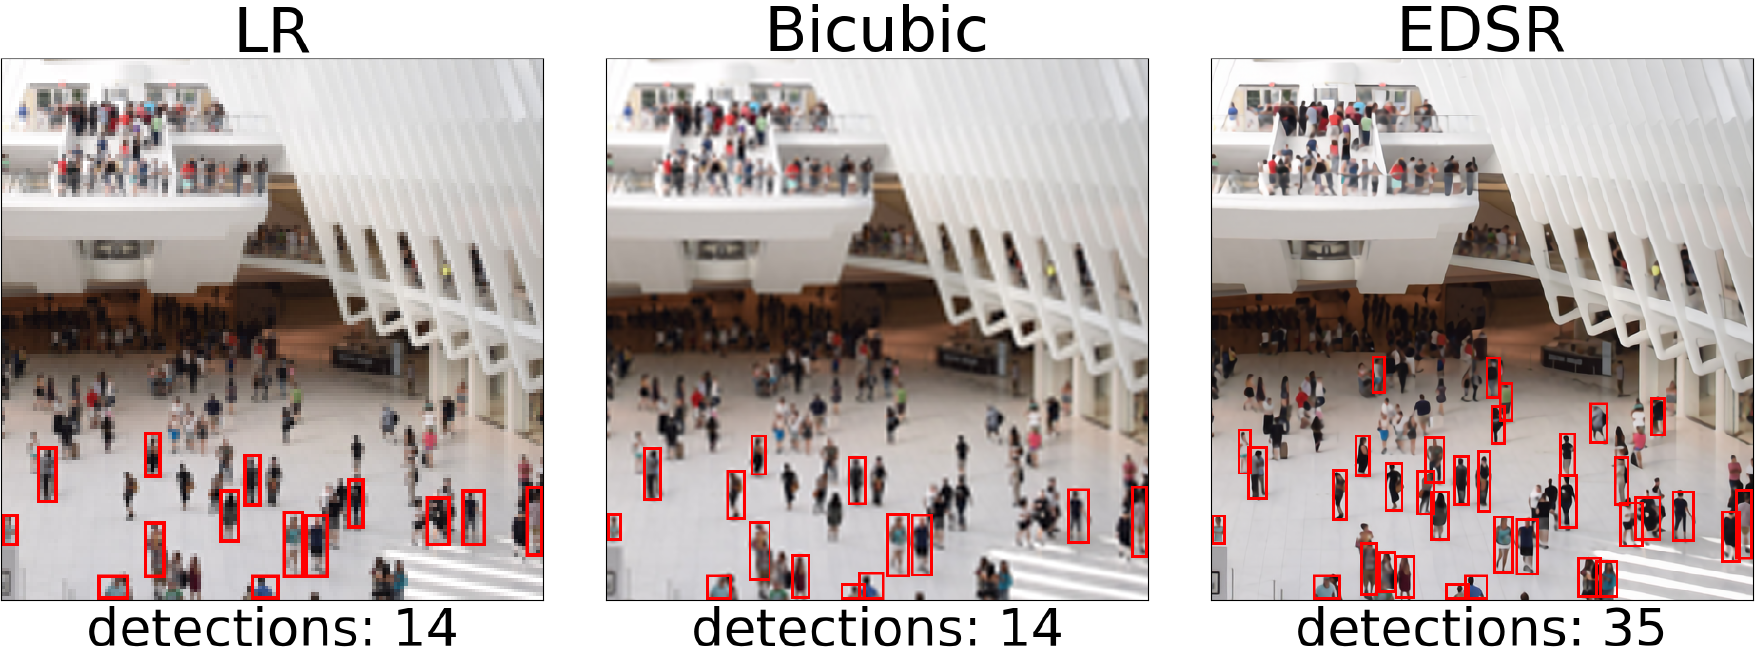
\includegraphics[width=0.85\textwidth]{yolo_people_sr.png}
\caption{YOLO people detections on a image ROI.
\textbf{(left)} The original ROI and its corresponding detections.
\textbf{(center)} Up-sampling of the original ROI using a bi-cubic algorithm and its corresponding detections.
\textbf{(right)} Up-sampling of the original ROI using the EDSR model and its corresponding detections.
The use of Super Resolution model is able to improve the YOLO detection of small persons of more than 200\%.
YOLO is not still able to detect the smaller (far) persons.
}
\label{fig:yolo_sr}
\end{figure}

On the first image (left) of Fig.~\ref{fig:yolo_sr} we show only a small ROI of the (larger) input image in which the YOLO model is able to identify only a small part of people.
We would stress that the detected people are all in the bottom of the image, in which the size of persons are bigger.
Using a standard bicubic up-sampling (center of Fig.~\ref{fig:yolo_sr}) the detection performances are the same and this proof as standard up-sample methods are not appropriate to overcome this task.
The application of EDSR model (right of Fig.~\ref{fig:yolo_sr}) is able to improve the quality of the image and ease the work of YOLO model.
In this case the detection is more than twice of the previous case.
The issue remains for the top of the image where only few pixels identify a person.
Set out to test the limit of this model combination we extract a further ROI from it selecting only the top part of the image.
The results are shown in Fig.~\ref{fig:yolo_sr2}.

\begin{figure}[htbp]
\centering
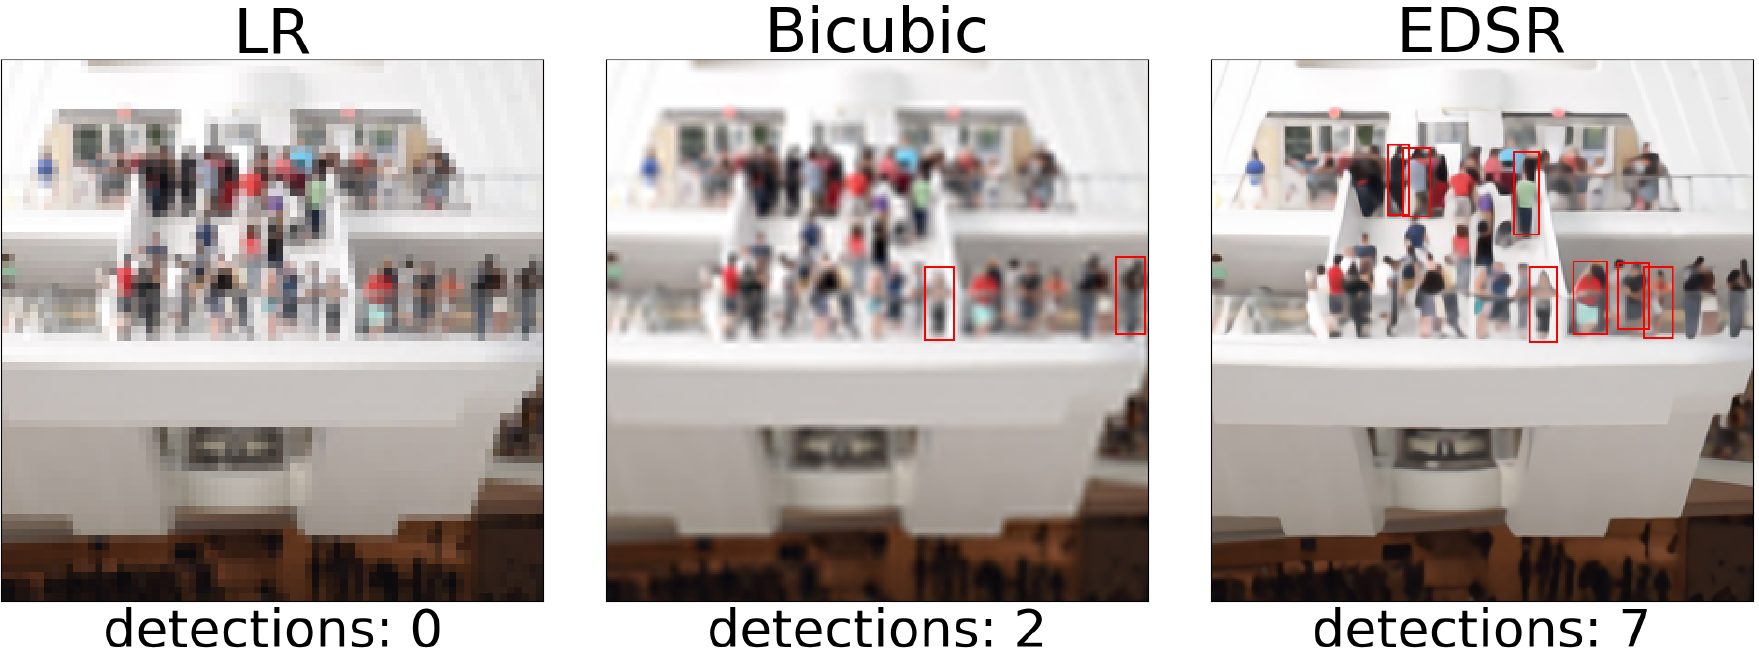
\includegraphics[width=0.85\textwidth]{yolo_people_sr2.png}
\caption{YOLO people detections on a ROI of the previous image ROI.
\textbf{(left)} The original ROI and its corresponding detections.
\textbf{(center)} Up-sampling of the original ROI using a bi-cubic algorithm and its corresponding detections.
\textbf{(right)} Up-sampling of the original ROI using the EDSR model and its corresponding detections.
Without the Super Resolution application the YOLO model is not able to recognize any person.
The bi-cubic up-sampling allows the detection of only 2 persons against the 7 obtained by the use of EDSR model.
}
\label{fig:yolo_sr2}
\end{figure}

The task in this case is certainly harder and also a human eye hardly count the number of persons into the image.
With the raw image the YOLO model is not able to identify anything and also with the bicubic up-sampling only 1 person is recognized by the model.
With the EDSR pre-processing the detection performance increases and 7 persons are recognized.
Certainly the people count is underestimated but the Super Resolution pre-processing seems to be the only available solution to improve the YOLO performances on these tasks.


\end{document}
